\section{Concept 2 - Component/structure editor}
This section presents the second requirement-to-test translation concept, proposes a rudimentary meta model and evaluates the approach in terms which parts should be refined in a later concept, and which shouldn't.
The second concept originated from the idea that structure, could be added by component-oriented tool. The user interface only provides graphical components that represent domain actors and concepts than can be connected and re-arranged to create the use cases. The user interface should then -- similar to the first concept -- providing immediate visual feedback in the form of textual use case representation (or a diagram), like in the first concept.\\\\\
The procedure of the concept is to define actors and concepts beforehand, and then compose use cases from these. So, if starting from scratch, a user would be expected to initially define at least one actor and the actions that the actor perform, and the objects that this action would -- prior to actually writing the use case.\\\\
\begin{figure}[!htbp]
\includegraphics[scale=0.4]{\imgdir test_case_ui}
\centering
\caption{Use case editor UI mockup}
\label{fig:use_case_editor_mockup}
\end{figure}A user interface mock-up is shown in figure \ref{fig:use_case_editor_mockup}. In the top of the screen is tab selector that navigates the selected use case. In the selected use case panel, we can see the main scenario (the selected tab), where the list use case entries are shown. The selected entry is ``Receptionist send Message'', which is also shown in the bottom of the user interface where it can be edited. The available actors and concepts are shown on the right side of the user interface. The pre- and postconditions are part of the user interface, but is included in the meta model discussion.\\\\
This concept was not chosen, due to the significantly increased workload that it involved, and the added complexity. The concept and its corresponding meta model was simplified, and was refined for the next concept.

\subsection{Meta model}
This section contains a brief discussion of a meta model that could be used for translating use cases into test cases in this concept. The discussion is supported by the graphical model depicted in figure \ref{fig:meta_model}, which show the concepts that are being discussed.

\begin{figure}[h]
  \centering
 
  \includegraphics[scale=0.72]{\imgdir concept2_use_case_meta_model}
  \caption{Intermediate meta model for use case representation along with tests}
  \label{fig:use_case_meta_model}
\end{figure}

The central point of the meta model is the use case. It is composed of stakeholders and a primary actor, pre- and post-conditions, use case entries (the Entry class) and a number of extensions. The primary actor is mostly for information purposes, as the Actor class (which models the domain actor) is also contained within the entries. The Entry class model the use case's entries, and are not very flexible as they expect a use case entry to consist of an actor, a target and an action. The target may be either a domain actor or a domain concept.\\
The extensions are treated as lists of use case entries as well as the main scenario. In addition; they have extension points as well as optional return
The pre- and postconditions are treated as en

%TODO update meta model.

% What you cannot do, when having two actors, is specify the direction of the action.

for now, we take a look at the ``Main success scenario'' and see that, broadly speaking, each use case action involves one actor performing an action, possibly affecting a target object -- which could be another actor. For the purpose of generating tests, it is not important that actors may target other actors though their actions, and this association is therefore left out of the meta model.\\\\
Postconditions are -- in this model -- defined to be predicates. This is because they share the common trait that they must be true, for the given expression to be true. In our case, the postcondition ``Receptionist is ready for next call'' states the actor receptionist that is participating in this use case, must be in a specific state when the last statement of the use case is done. A postcondition should refer to an actor, target or action previously defined in the use case to avoid redundant mapping. The predicate itself can be some sort of quantifiable strict logic such as ``Message has recipients'', or could as an extension be defined as the more loose ``Message should have recipients'', which should map to a warning in the generated tests, rather than an error.


\\\\
Within the definition mapping, the mapping class denotes the relation between either a predicate and a predicate expression, or a statement (indirectly by the actor, action, target composition). The mapping is uniquely defined by mapping by its composition of an actor, an action and a target, as it should be safe to assume that ``The contact accepts the call'' means the same no matter which use case it appears in. Each mapping will imply a requirement on a resource, which can be any actor or target. The are basically constraints stating the minimum functionality the test framework\footnote{Domain-specific scaffolding code that needs to be written by hand} should have to make the generated test code runnable. These resources could, in test code frameworks, be provided by factory classes or object pools.\\\\
Tests are the output of a sequence of mappings, that has a state which is then defined by the mappings that originally defined the test. The test will also have references to the predicate expressions that are outputted by mappings as well.



Pre and post-conditions are operations that work on expressions rather than statements

Alternate scenarios are not yet covered.

\subsection{Meta model}

\begin{figure}[h]
  \centering
 
  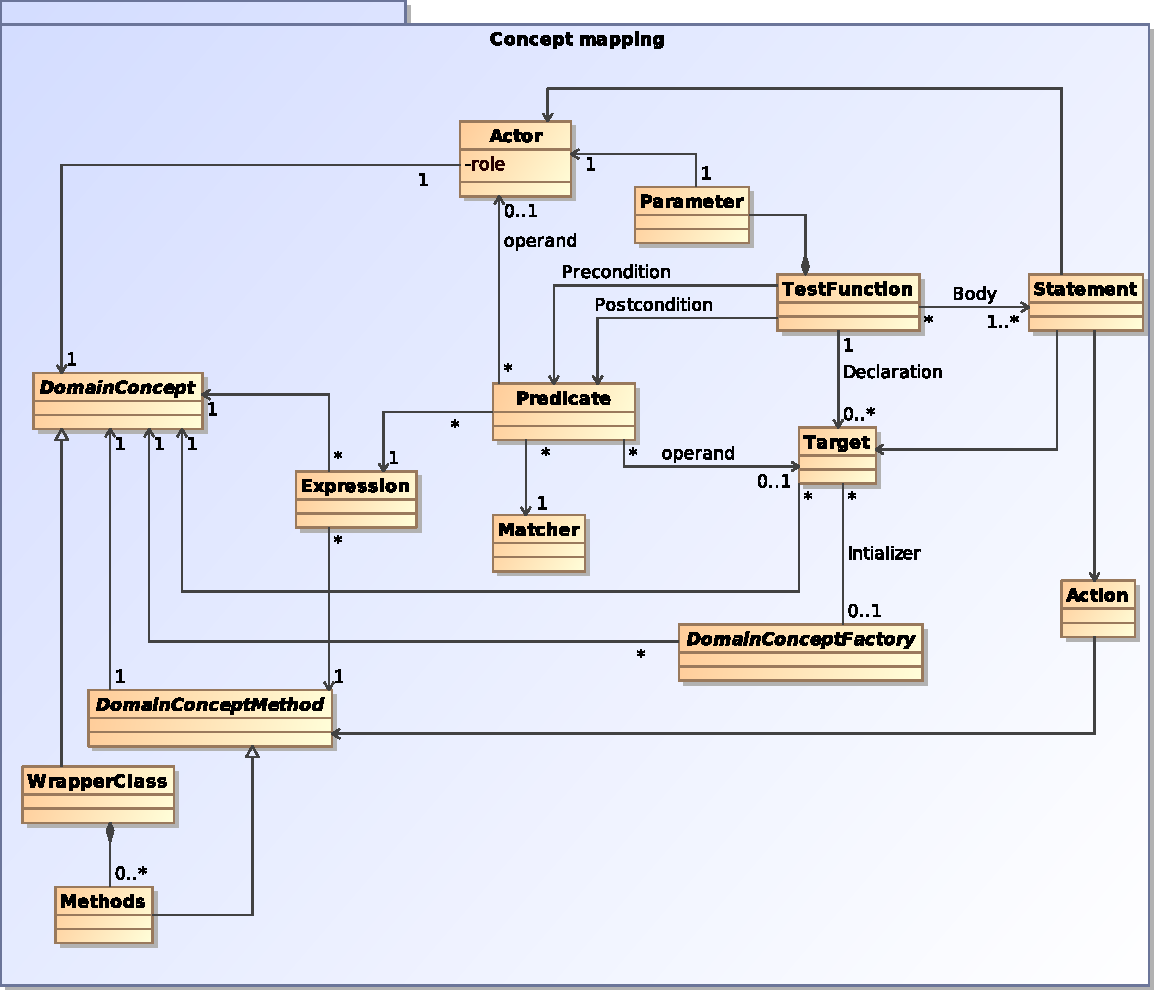
\includegraphics[scale=0.72]{img/use_case_mapping}
  \caption{Use case mapping}
  \label{fig:use_case_mapping}
\end{figure}

\section{Mapping manually}
Within a use case there are some bits of implicit knowledge that we need to extract. To begin with, we observe that for the use cases in figure \ref{fig:uc1} and \ref{fig:uc2}, there are domain actors involved.

Each involved domain actor will then be mapped to a wrapper class that represents the domain object, and could possibly extend a class from the implemented code base.

In order to get the actor object to perform actions, we need to map the actions in the use case to some functions associated with the actor class. These functions could be a direct link to a method that is part of the main codebase which is tested against, a new method written specifically for this purpose - or a macro function that combines functionality from different domain concepts in a single functions.

Whenever there is a mention of an object (a target of an action) which could be, for instance, a message object we assume that its the same object that is tracked during the entire use case. So, from use case 2, we have ``Receptionist sends the message via the system'' in the main success scenario and ``Message is stored and ready for dispatching'' in the postconditions.

So, summing up, we have in this model a very strict view on single use case entries:
\begin{itemize}
  \item This use case consists of an ordered list of actions, where actions consist of
  \begin{itemize}
	\item One or more actors
	\item One verb describing the action
	\item One target for the action (object for verb)
  \end{itemize}
\end{itemize}
If we 


One of the problems with this solution is that you also need to specify who is performing the action, and who is the target.
\subsection{Evaluation}
It was too far from acutally writing the use cases. Having to decompose the use case before acutally wiritinh it is not very user friendly. 
A big problem with this approach is that it could quickly lead to artificial or too technical jargon in use cases, which is generally a bad idea as it alienates the customer \cite{christel1992}.
%TODO What are the good parts?